\documentclass[../main.tex]{subfiles}

\begin{document}
\section{CHIPS Architecture}
The CHIPS architecture is an amalgamation of heterogeneous chiplets connected through an interposer package, and the AIB allows the chiplet to communicate through this package\cite{AIBWhitePaper}. There are two layers on the protocol stack. AIB is the lowest level in the stack, and AXI is the upper level in the stack. All chiplets use AXI as the memory transfer protocol.

In phase one, there is no interposer, so AIB drivers connect through standard metal layers. The Rocket chiplet is the only chiplet to have AIB, due to time constraints For risk mitigation on the AIB, there are two Rocket chiplets, one with AIB and the one without AIB. 

The following is a list of combined technologies and groups of people or organizations involved in implementing sed technologies. The AXI bus structure uses the Pulpino AXI IP. Dr. Lee Baker and Dr. Summon Dey provided the LSTM chiplet. Dr. Lee Baker and Dr. Weifu Le provided the SCNN chiplet. Joshua Stevens provided the modified Rocket chiplet, initially from UCB. Tse-Han Pan and Joshua Stevens provided the Rocket chiplet with AIB. Tse-Han Pan provided the physical IP for the AIB drivers, initially from Intel. Dr. Lee Baker and Dr. Joshua Schabel provided the modified IP for the AIB channel. Joshua Stevens, Dr. Lee Baker, and Dr. Steve Lipa provided the top-level IP. Dr. Lee Baker provided CIPI to AXI bridge and on-chip memory controller. 

\subsection{AIB Structure}
The AIB interface allows each chiplet to connect to the interposer package. The physical chiplet to interposer to chiplet package layout is in figure \ref{fig:AIBInterposer}. On each bump, there is an AIB driver, and this driver is capable of running at a single data rate (SDR) or double data rate (DDR)  \ref{fig:AIBInterposer}. SDR is the configuration used in this architecture. Two sets of AIB drivers work in pairs, one set to transmit and the other set to receive. A group of drivers makes up an AIB channel, and in each channel, there are at least the following singles: Tx to Rx, clock transfer, and control transfer\ref{fig:AIBInterposer}. The typical configuration for a channel is in figure \ref{fig:AIBInterface}. Two AIB channels form the AIB interface, one channel is a master and the other a slave  \ref{fig:AIBInterposer}. In each channel, each bump connects to its corresponding bump on the other side of the interface. Figure \ref{fig:AIBChannel} shows this connection structure.  

\begin{figure}
    \centering
    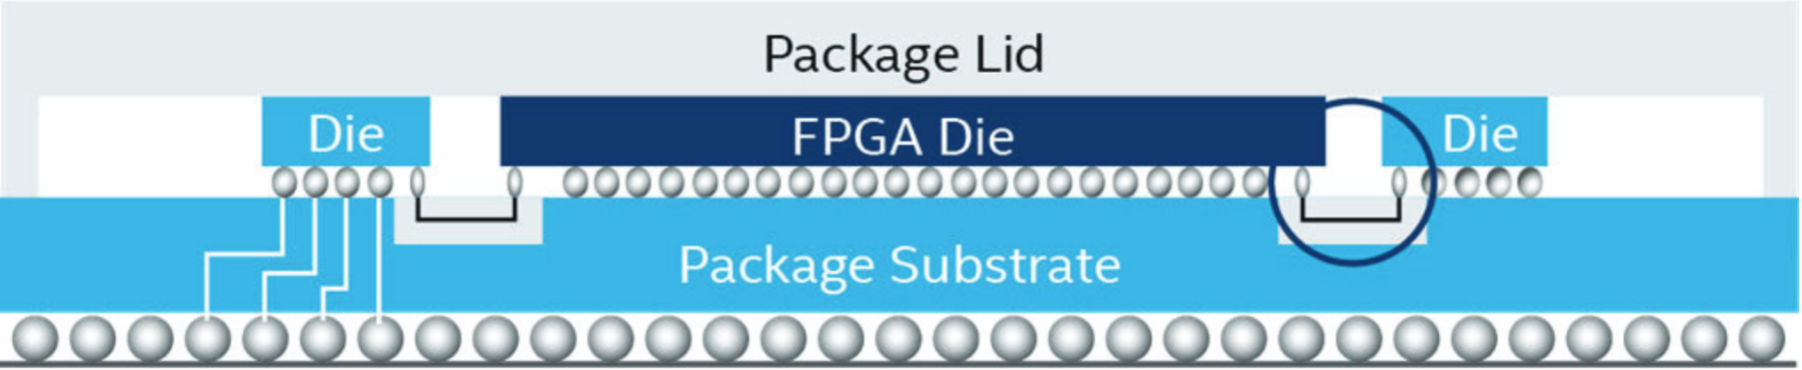
\includegraphics[scale=.25]{pngs/Interposer.png}
    \caption{AIB Interposer Connection\cite{AIBWhitePaper}}
    \label{fig:AIBInterposer}
\end{figure}
\begin{figure}
    \centering
    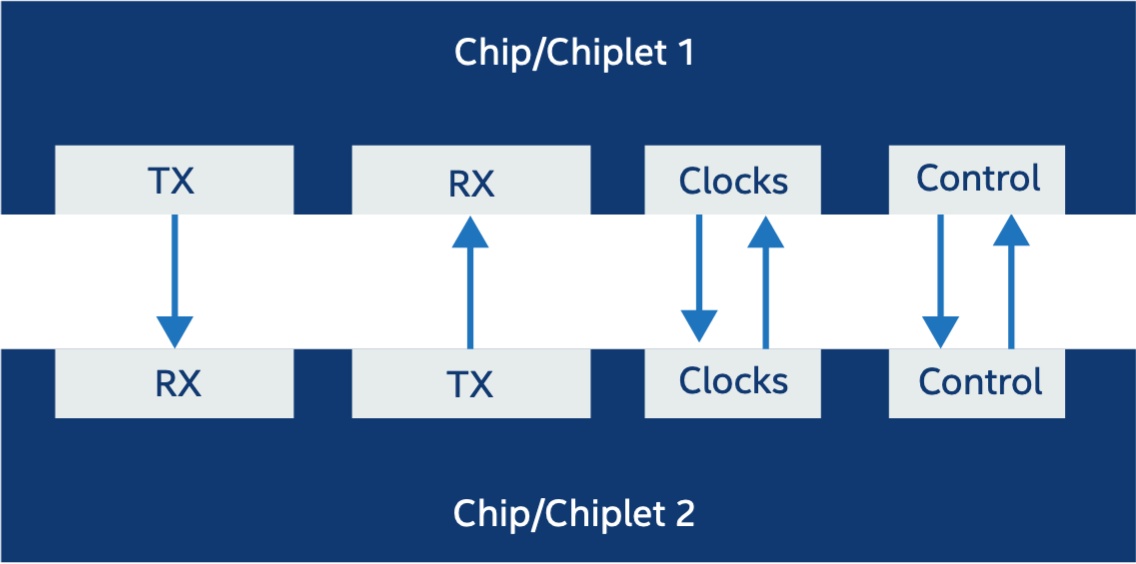
\includegraphics[scale=.32]{pngs/AIB-interface.png}
    \caption{AIB Interface\cite{AIBWhitePaper}}
    \label{fig:AIBInterface}
\end{figure}

\begin{figure}
    \centering
    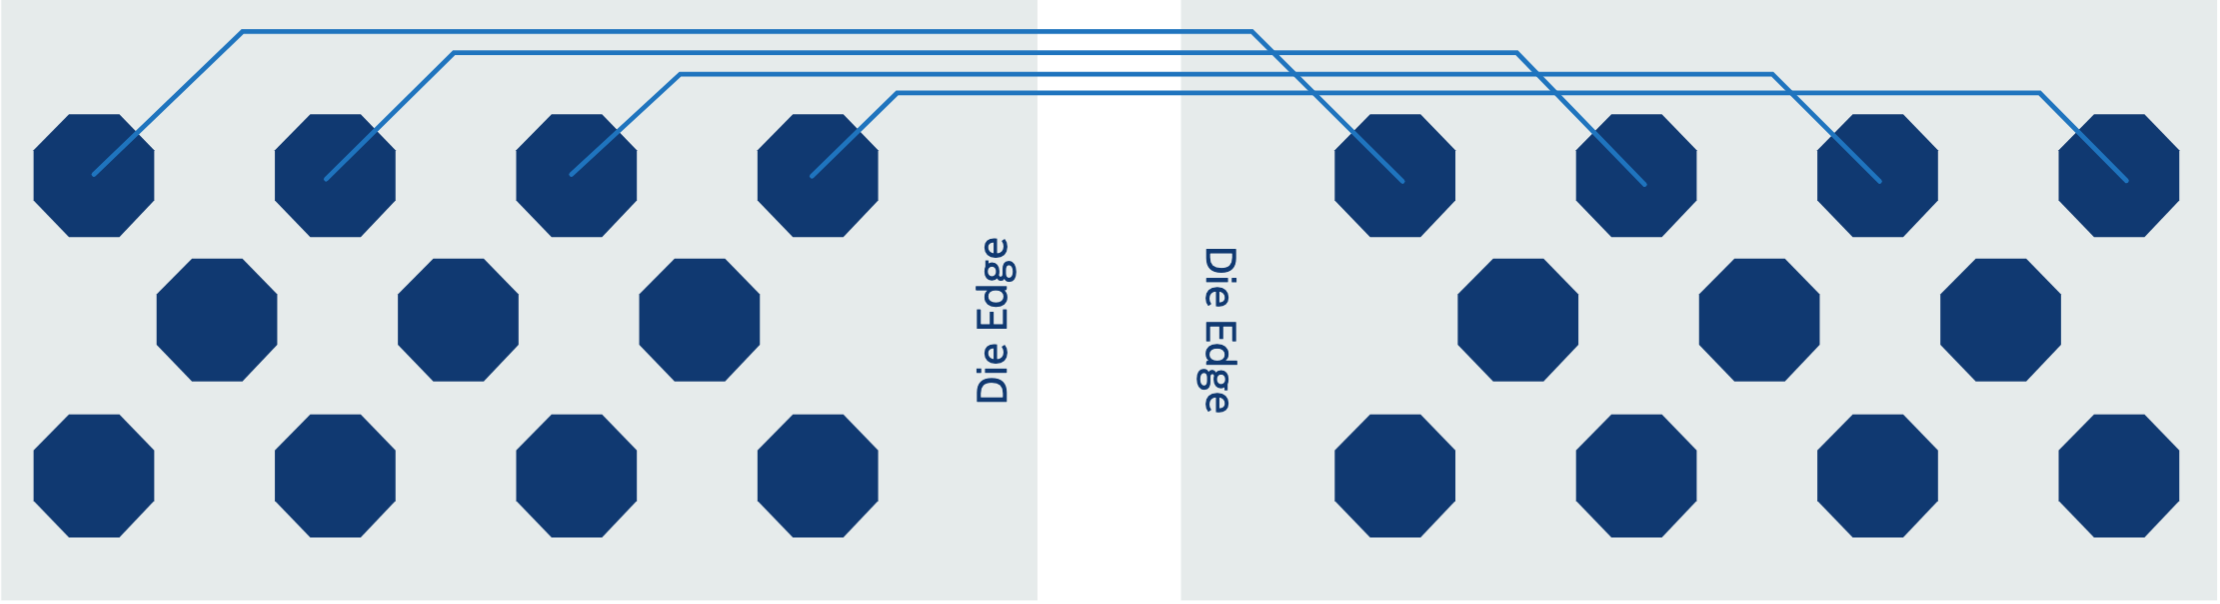
\includegraphics[scale=.17]{pngs/AIB-Channel.png}
    \caption{AIB Channel Connection\cite{AIBWhitePaper}}
    \label{fig:AIBChannel}
\end{figure}

 For this architecture, 48 AIB drivers make up an AIB channel. Each channel has the following functions: clock transfer, data transfer, and there is no control transfer in this implantation. The data transfer is in the lower 40 drivers, and clock transfer is in the upper eight drivers. For clock transfer, two drivers are used to transmit a differential clock \ref{fig:AIBInterposer}. This grouping makes up four clock functions. Each of the four clocks is divided up into two types of functions: master data transfer and slave data transfer \ref{fig:AIBInterposer}. The data transfer function requires two sets of differential clocks. For this function, one clock launches on one side of the interface, and then it is received and looped back on the other side, and finally, it gets received on the same side that launched the original clock \ref{fig:AIBInterposer}. This group of clocks forms the clock loop-back functionality needed to synchronize data from master to slave, and vise versa \ref{fig:AIBInterposer}. The following figures show the different driver functionalities: Transmit functionally figure \ref{fig:AIB-Tx}, loop-back functionally figure \ref{fig:AIB-Rx-Tx} and receive functionally figure \ref{fig:AIB-Rx}. 

\begin{figure}
    \centering
    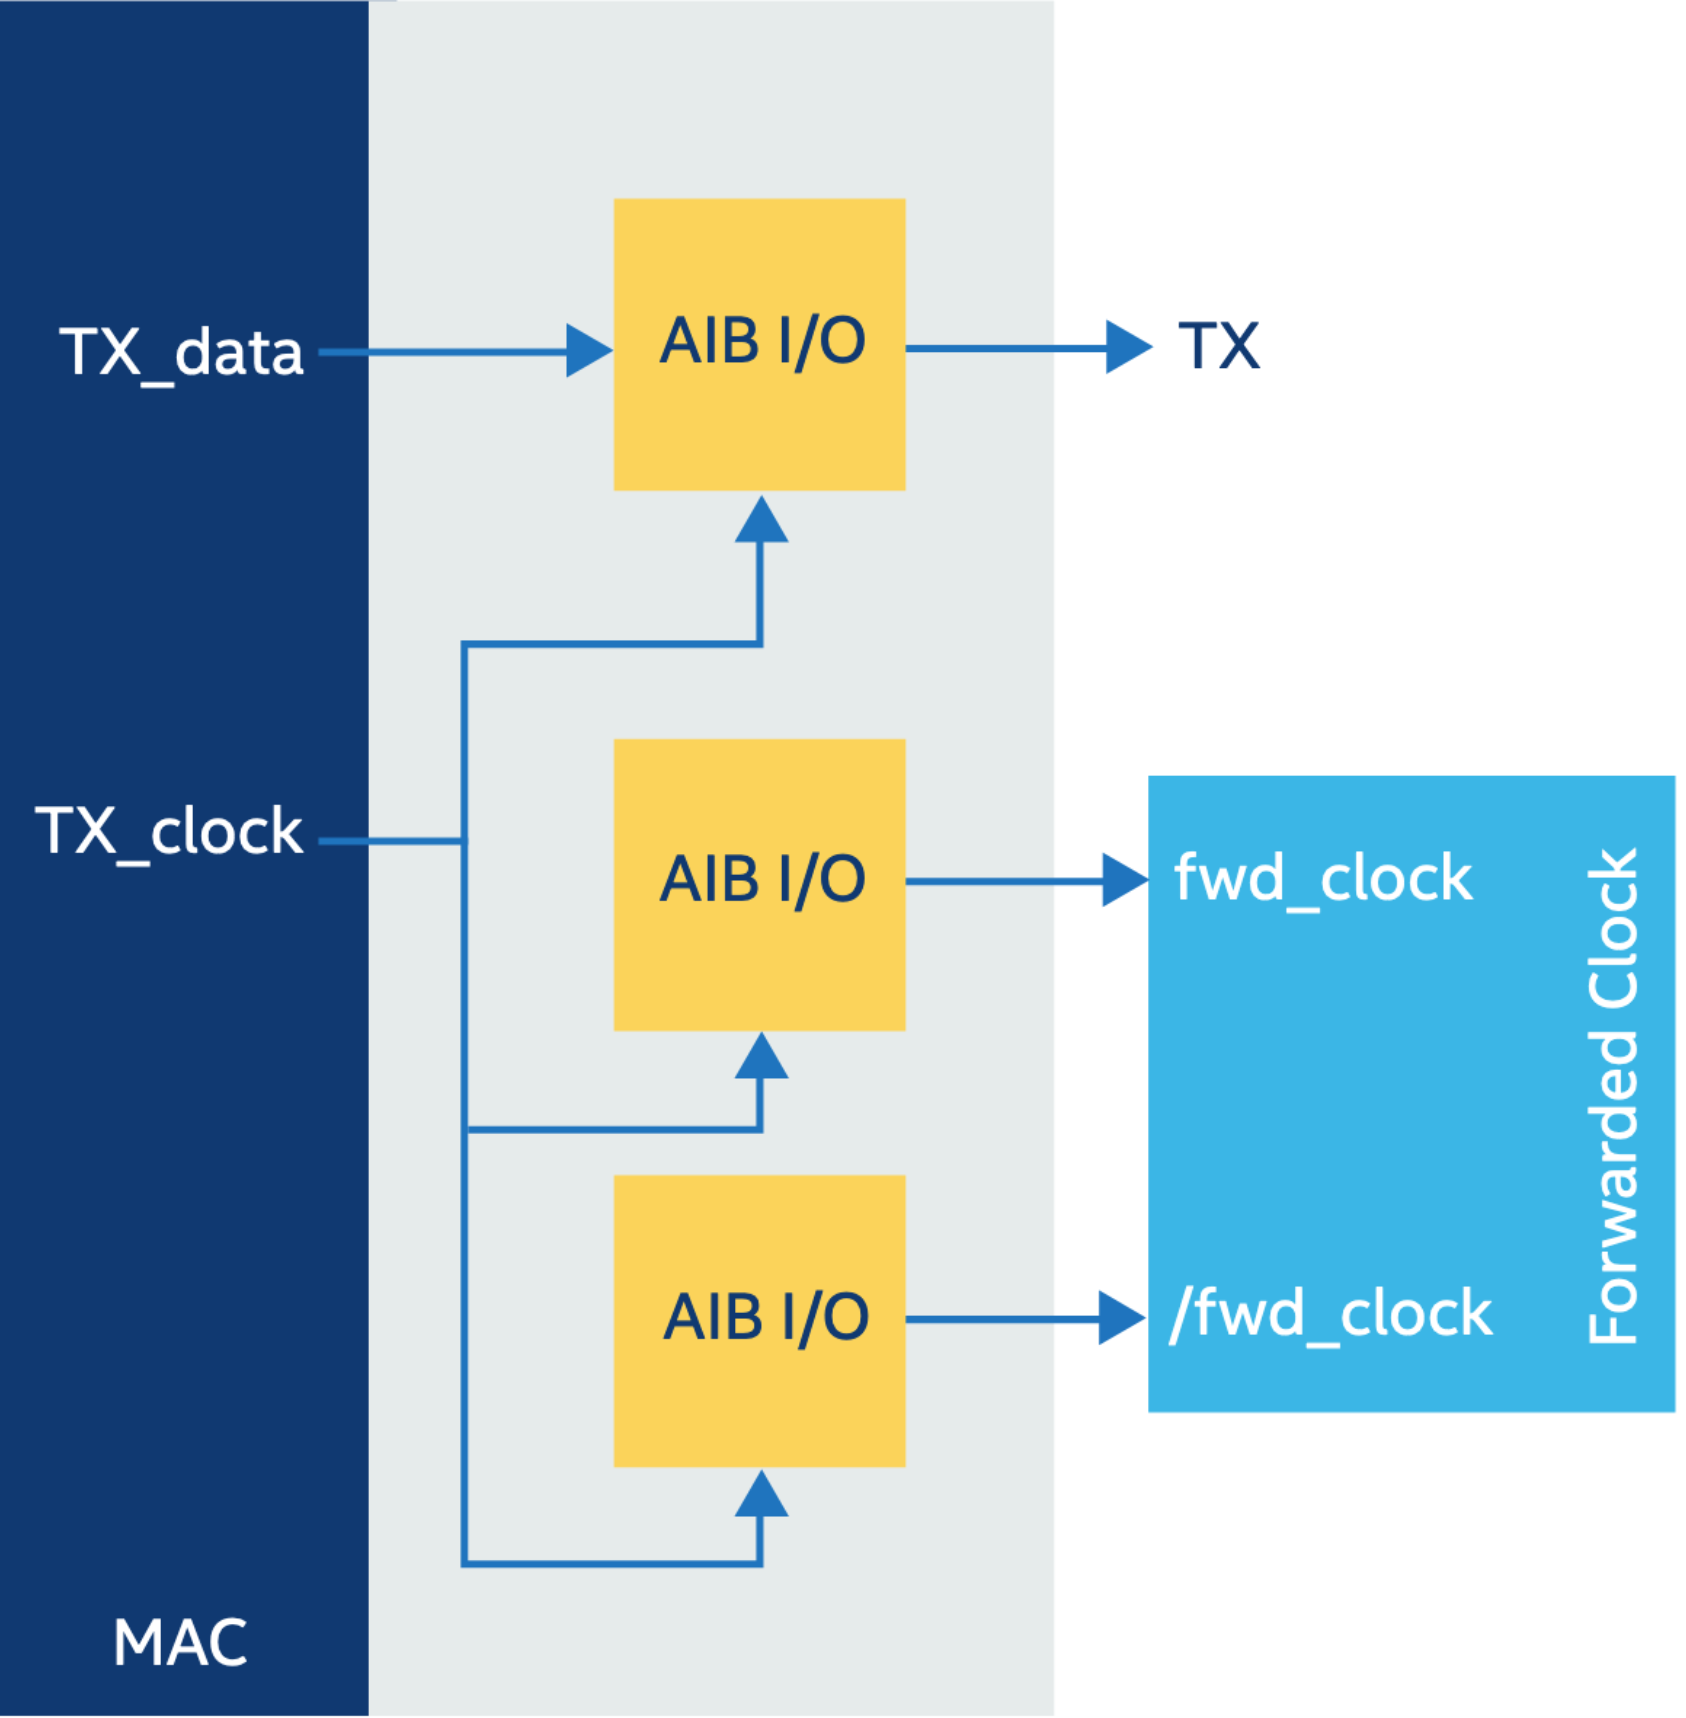
\includegraphics[scale=.16]{pngs/AIB-Tx.png}
    \caption{Transmitting\cite{AIBWhitePaper}}
    \label{fig:AIB-Tx}
\end{figure}

\begin{figure}
    \centering
    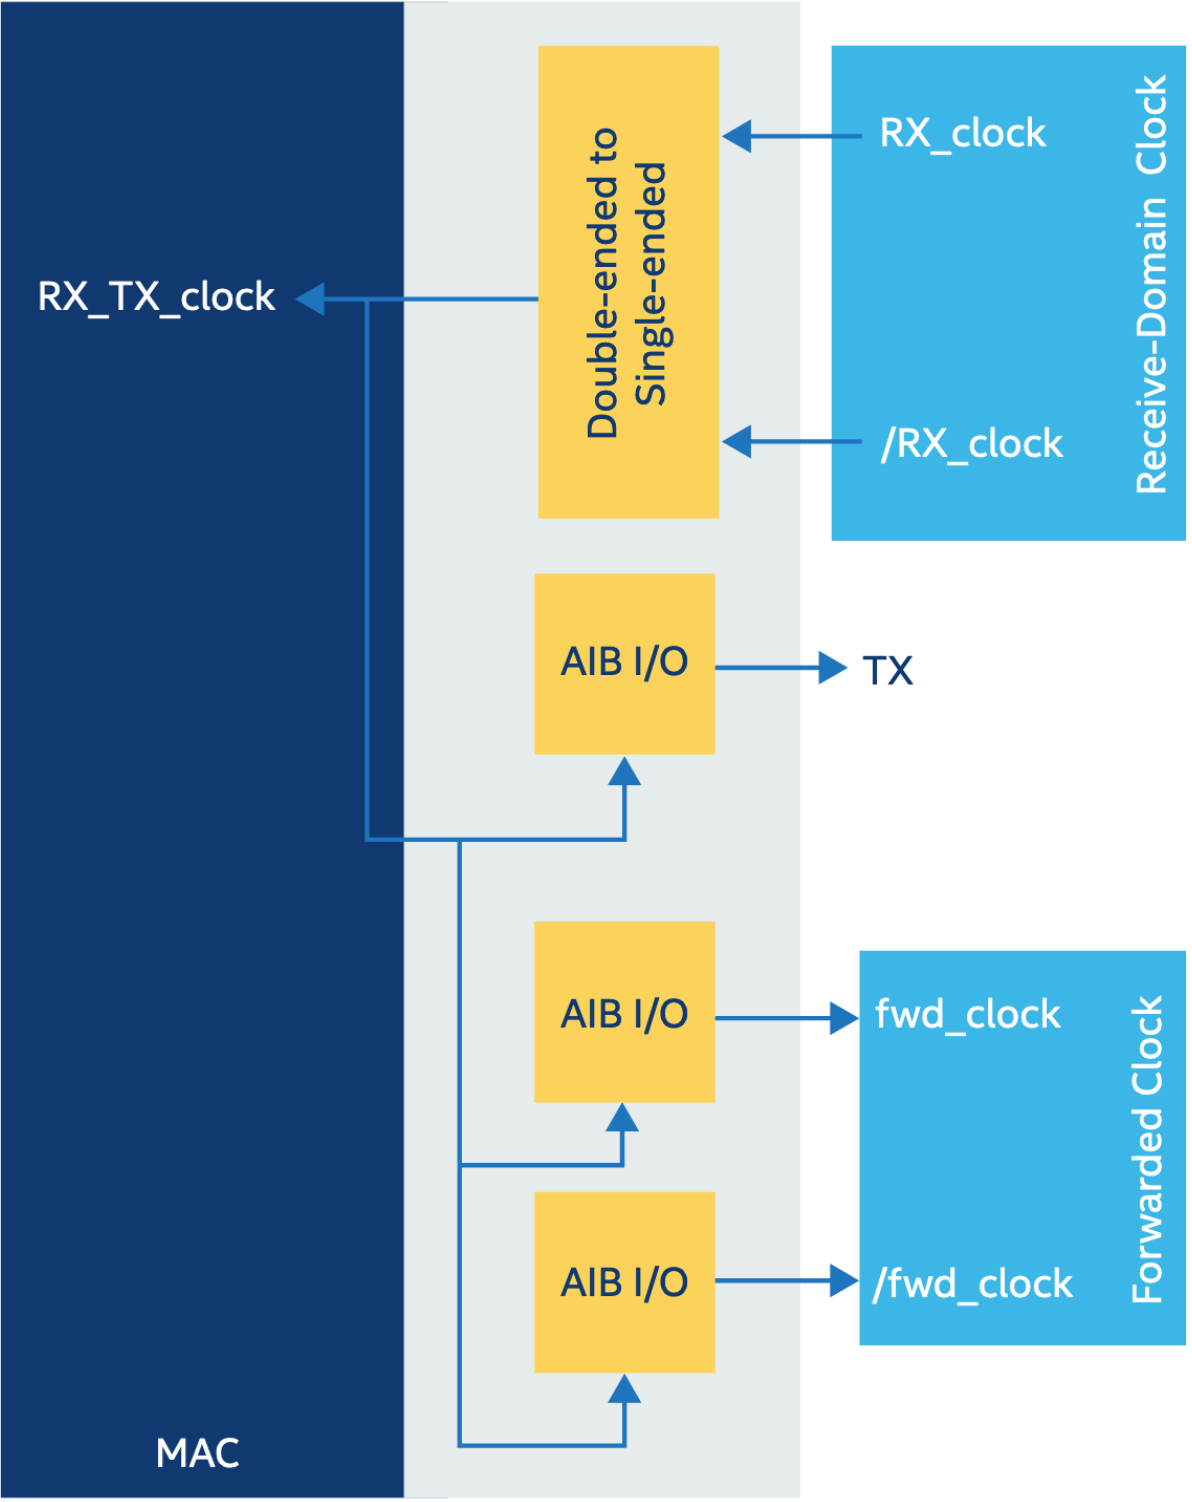
\includegraphics[scale=.2]{pngs/AIB-Rx-Tx.png}
    \caption{Forwarding\cite{AIBWhitePaper}}
    \label{fig:AIB-Rx-Tx}
\end{figure}

\subsection{CHIPS SOC}

\begin{figure}
    \centering
    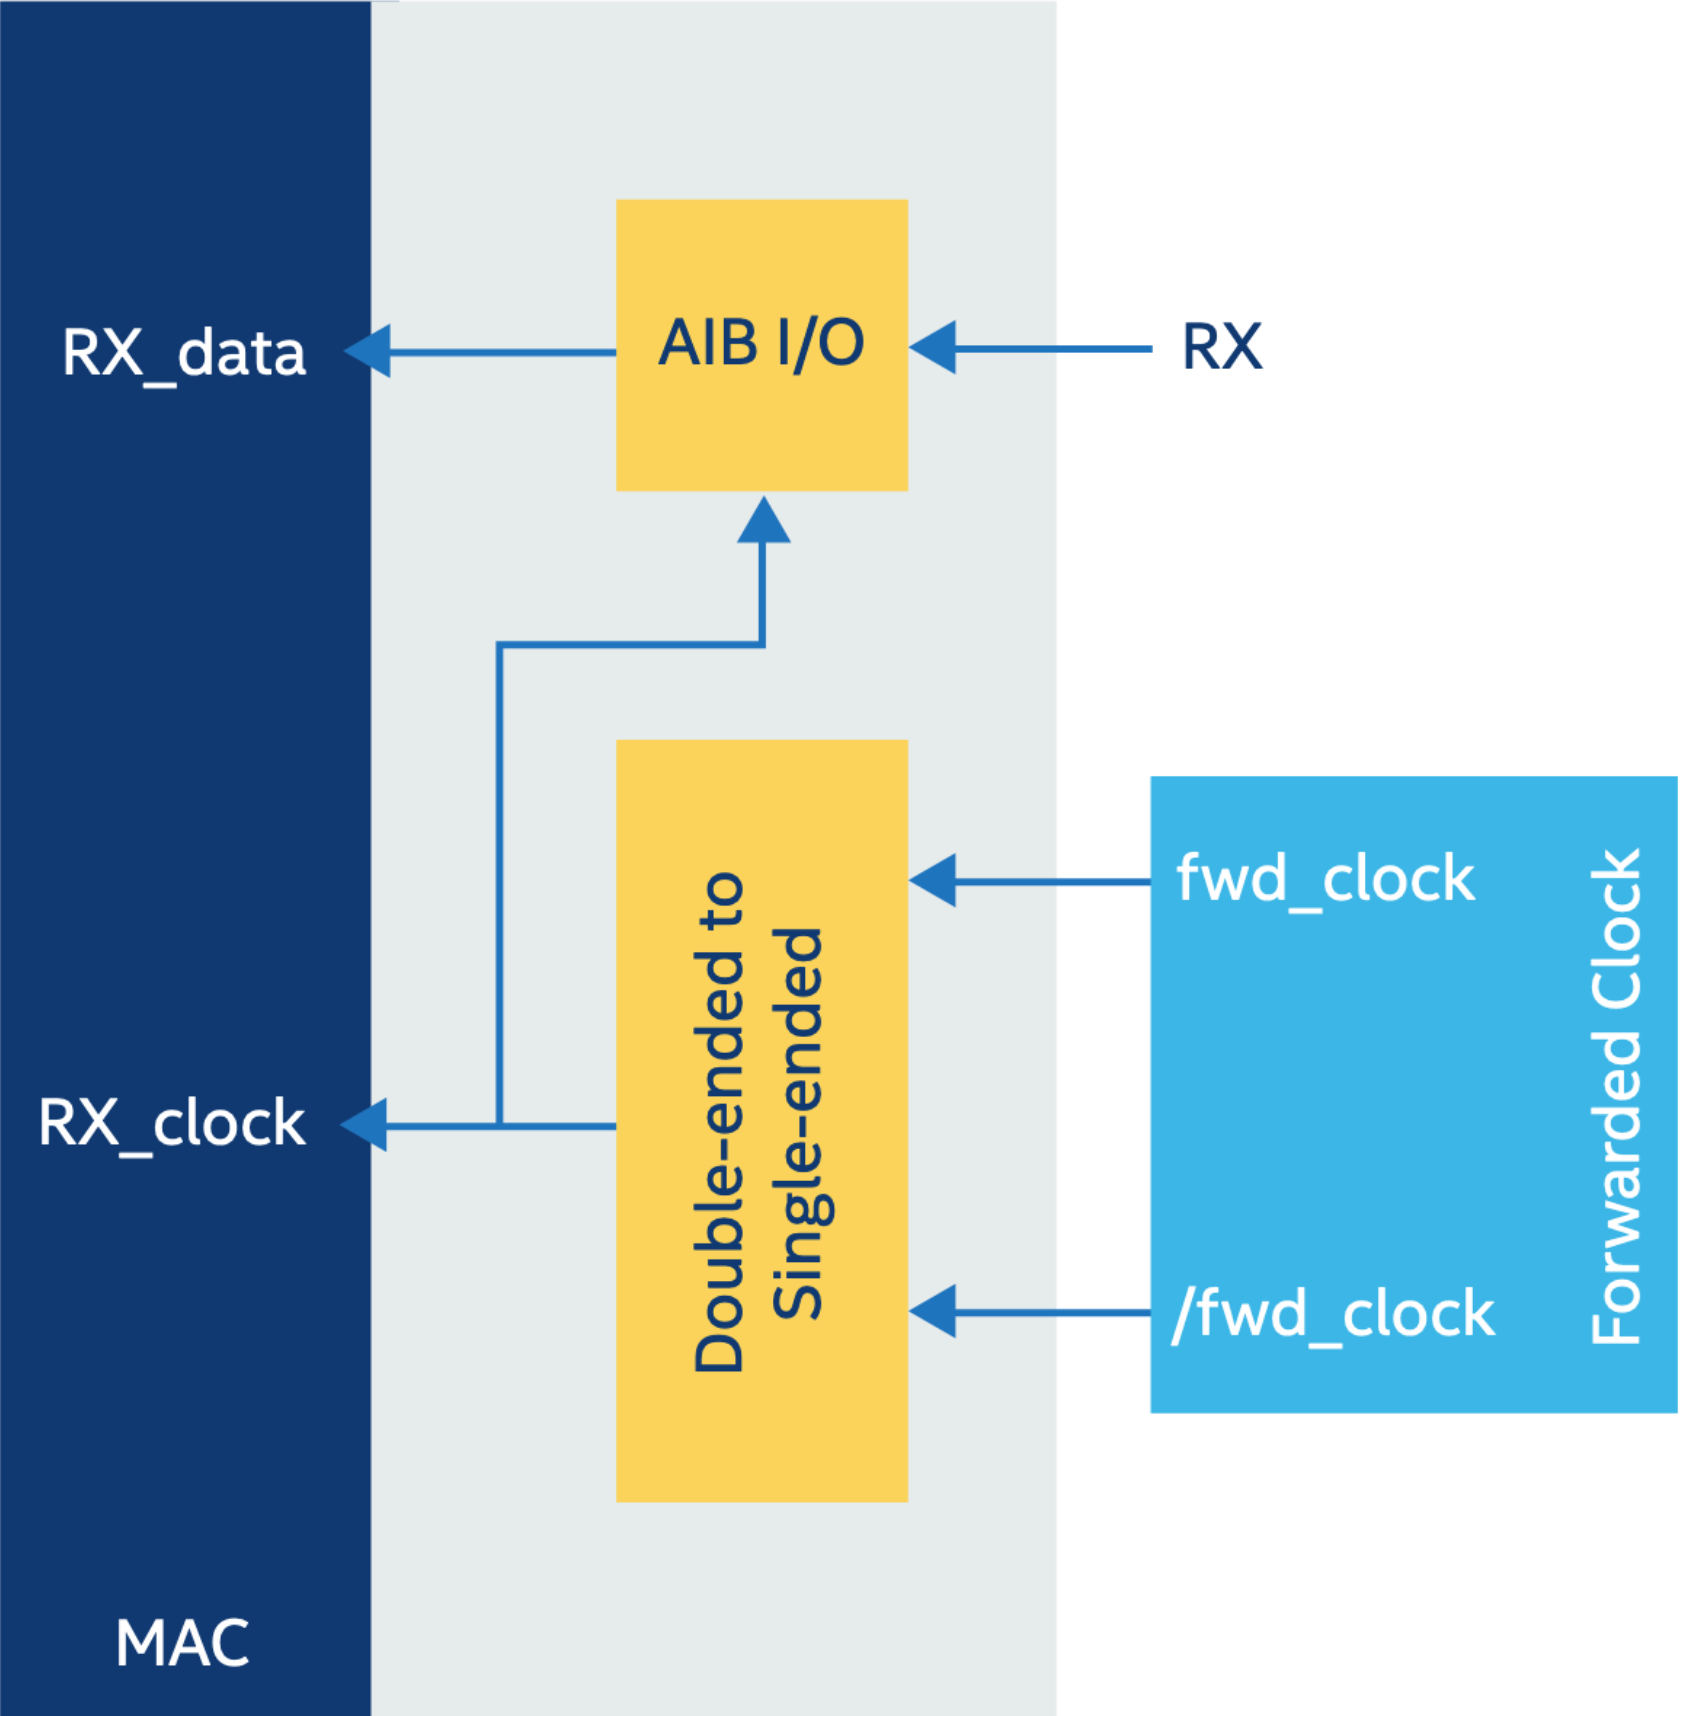
\includegraphics[scale=.16]{pngs/AIB-Rx.png}
    \caption{Receiving\cite{AIBWhitePaper}}
    \label{fig:AIB-Rx}
\end{figure}

\begin{figure}
    \centering
    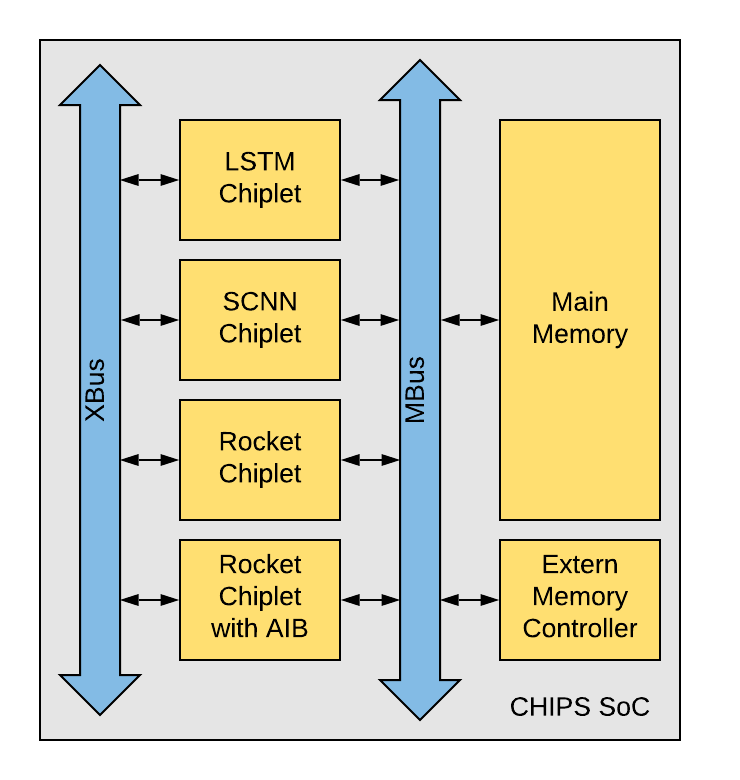
\includegraphics[scale=.45]{pngs/CHIPS-system.png}
    \caption{CHIPS SOC}
    \label{fig:CHIPS-arch}
\end{figure}

The CHIPS SoC consists of two bus types, debug (JTag) and memory (AXI). JTag allows interactive control over the chiplets and the SoC sub-system. The SoC contains two AXI bus: one is for on and off-chip memory access (MBus), and the other is for neural network chiplet control (XBus).  The Mbus allows each chiplet to connect to the on-chip memory. The external memory controller bridges the MBus with the off-chip memory bus(ExMBus), and this bus uses the Custom IP Interface (CIPI) protocol. The XBus allows the Rocket chiplets to control the behavior of the neural network chiplets. Figure \ref{fig:CHIPS-arch} shows an overview of the Chips SoC(Jtag ports omitted for visibility).


\subsection{Chiplets}
Each chiplet has three bus connections. Controller chiplets, Rocket chiplets, has two master AXI ports, XBus and MBus, and one JTag debug port. Neural network chiplets, has one master AXI port, MBus, one slave port AXI port, XBus, and one Jtag debug port.

\subsubsection{Rocket Chiplet}
The Rocket chiplet had to be modified to work within the CHIPS architecture. The default Rocket chiplet has only an AXI memory port at the L2 cache level, and this structure was modified not to include an L2 cache. Now the Rocket chiplet has only one AXI port at the L1 cache level. In addition to the L1 AXI memory port, another AXI memory port is needed to access the XBus. To access the XBus, the RoCC AXI bus controller replaced the default RoCC unit, and this controller allows the Rocket chiplet to control the neural network chiplets through the XBus. The floating-point unit (FPU) was not needed. In addition to the AXI bus controller, the Rocket chiplet's Jtag had to be modified to support the ability to control the AIB channel's configuration registers.

\subsubsection{Neural Network Chiplets}
In this architecture, there are two neural network chiplets: LSTM and SCNN. Both chiplets are accessible via JTag port or XBus port. These chiplets are designed to work at the coarse grain programming level. 

The LSTM chiplet is the product of Dr. Summon Dey's dissertation research at NCSU\cite{Summon-Dey-LSTM}. The LSTM chiplet focuses on developing hardware that can fully utilize its memory bandwidth. Dey's chiplet scales with the amount of memory bandwidth available. The chiplet must also be able to adapt to changes in recurrent neural networks (RNN) algorithms. To this end, he based his design on a very long instruction word (VLIW) architecture. In this style of architecture, a single instruction represents a set to micro-opts. Each micro-opt controls a section/lane of the design. See his paper for more details on his design\cite{Summon-Dey-LSTM}.

The SCNN chiplet is the product of Dr. Weifu Li's dissertation research at NCSU\cite{LeWeifuDissertation}. His chiplet design focuses on reducing the amount of memory access needed to process a CNN. To this end, he uses a run-length encoding (RLE) format to compress the zeros in the input feature data and weights. His hardware uses the RLE data to reduce the amount of memory access to memory.

\end{document}

